\begin{abstract}
Pairwise leaderboards turn comparison outcomes into an ordered list, but the stability of that list depends on both the observed evidence and the fitted model. We audit retrospective outcome-flip sensitivity in public Chatbot Arena preferences, MT-Bench human and GPT-4 judgments, and ten NBA regular seasons. We reverse distinct decisive outcomes while preserving comparison schedules and ties, then refit a ridge Bradley--Terry model. Influence-guided searches find reversals of the original leading pair after 2 of 57,477 Arena outcomes, 46 of 3,355 MT-Bench human judgments, 61 of 2,400 GPT-4 judgments, and 1--8 games per NBA season. These are successful-edit upper bounds, not minimum budgets. Arena and every NBA leading-pair bootstrap interval already include zero; the two MT-Bench intervals exclude it. On identical MT-Bench comparison cells, a paired question bootstrap gives a mean human-minus-GPT-4 found edit fraction of $-1.20$ percentage points, with a descriptive percentile range of $[-2.24,-0.11]$ points for a fixed reference pair. Sensitivity also changes with tie handling and regularization. The results support reporting edit witnesses alongside sampling uncertainty and modeling conventions; they do not establish that an evaluation design is inherently more vulnerable or that retrospective flips are operational attacks.
\end{abstract}

\section{Introduction}
A pairwise leaderboard can display a precise ordering even when the evidence separating neighboring entries is weak. This matters when a first-place label informs model selection, publicity, or scientific comparison. A small change to an outcome may have a negligible effect on fitted scores yet reverse a nearly tied pair. Conversely, a leaderboard with a modest sample can retain its leading contrast under many changes if that contrast is well separated. Counting edits alone therefore does not explain what a rank reversal means.

We study the following operational question: how do fitted rankings change when a small number of observed decisive outcomes are reversed, with the comparison schedule held fixed? Such an intervention can represent a sensitivity diagnostic for miscoded outcomes or deliberately chosen changes. It does not assume that anyone can edit an actual platform's history. We compare uniform random reversals, a simple targeted baseline, and an influence-guided search, measuring all reported effects with full model refits.

Our evidence covers crowd votes, human judgments on a fixed benchmark, model judgments on that benchmark, and sports results. These are deliberately different settings. We do not interpret the differences as effects of evaluation design: sample size, competitors, gaps, ties and schedules vary together. A matched MT-Bench comparison narrows the question by fixing the observed question--pair--turn cells and comparing label sources on the same support.

This paper contributes an empirical audit with three linked measurements: explicit successful edits to a selected leading contrast, random-perturbation and whole-ranking responses at matched fractional budgets, and cluster-bootstrap uncertainty before any edits. We also examine regularization, tie conventions, entrant coverage, human annotation subsets, and home advantage. The contribution is the jointly qualified evidence across these snapshots, rather than a new estimator or an optimal attack algorithm. In particular, ``two edits'' describes one fitted Arena snapshot under one convention; it is not a universal robustness threshold.

\section{Related work}
\label{sec:related}
Bradley--Terry models aggregate pairwise outcomes into latent strengths \citep{chiang2024arena}. Chatbot Arena operationalizes human preference comparisons for language-model evaluation \citep{chiang2024arena}, while MT-Bench provides human and model judgments that permit comparisons between label sources \citep{zheng2023judging}. We analyze the supplied public snapshots rather than reconstruct the platforms' current production rankings. In particular, our unweighted empirical-schedule ridge fit differs from Arena's reported inverse-sampling-weighted estimation for a uniform pair distribution, and our selected-gap bootstrap does not reproduce its simultaneous ranking-uncertainty procedure.

Influence functions approximate how a fitted quantity responds to small changes in observations \citep{koh2017influence}. Finite-sample robustness work asks whether changes to a small portion of a dataset can alter a substantive conclusion \citep{broderick2020amip}. Our use is narrower: a first-order score ranks candidate outcome reversals, and exact refits establish the resulting selected-pair changes. The candidate ordering is a computational heuristic, not a global robustness certificate. We preserve rows and participants, so results for deletion, reweighting, or vote injection are not interchangeable with this intervention. Huang et al. study influence-guided deletion sensitivity in Bradley--Terry leaderboards and validate candidate deletions by refitting \citep{huang2025dropping}. We therefore do not claim the first demonstration of leaderboard sensitivity or introduce influence-guided ranking audits. Our outcome-flip intervention retains ties and comparison schedules, uses a specified ridge fit, adds sports seasons, and places successful witnesses beside random perturbations and baseline uncertainty. Min et al. study new-vote injection under platform information and access constraints \citep{min2025rigging}; changing existing labels in a frozen dataset does not evaluate that operational threat model. Evaluation-policy questions, including selective disclosure and unequal sampling, are another distinct concern \citep{singh2025illusion}; our fixed-schedule experiments do not test those mechanisms. Published deletion or injection thresholds are not treated as newly executed numerical baselines.

\section{Question, estimands, and method}
\label{sec:method}
\paragraph{Data and fitting convention.}
An observation contains two participants $a_i,b_i$ and a canonical outcome $y_i\in\{0,\tfrac12,1\}$. The first participant wins when $y_i=1$; a tie contributes half a win. For $x_i=e_{a_i}-e_{b_i}$ and $p_i=\sigma(x_i^\top\theta)$, we minimize
\begin{equation}
 L(\theta)=\sum_{i=1}^{N}\left[\log(1+e^{x_i^\top\theta})-y_i x_i^\top\theta\right]+\frac\lambda2\|\theta\|_2^2.
 \label{eq:bt}
\end{equation}
We use $\lambda=1$ and centered logit scores in the primary study. The loss is summed, not averaged, so this convention must be specified when comparing sample sizes. Ties are fractional outcomes, not a fitted tie-probability model. Positive ridge yields a unique fit and controls separated or weakly supported competitors. Newton updates with line search are checked for convergence; every reported primary comparison graph is connected.

\paragraph{Intervention and budget.}
Choose distinct decisive rows $S$ and replace $y_i$ with $1-y_i$ for $i\in S$. Participants, row count, schedule, and all ties remain unchanged. We report the absolute count $k=|S|$ and $k/N$, where $N$ includes ties. Using all rows makes the denominator explicit across datasets with different tie rates; it does not make their information content equivalent. We also provide decisive-row counts. Curve budgets are one edit and $\max(1,\lfloor qN\rfloor)$ for $q\in\{0.001,0.0025,0.005,0.01,0.02,0.05\}$. Candidate exhaustion uses at most the stated budget and records the actual count.

\paragraph{Conditional and global endpoints.}
Select the initial leader $\ell$ and runner-up $r$ once from the original fit. The primary endpoint is reversal of $g=(e_\ell-e_r)^\top\hat\theta$: after refitting, $\theta_r>\theta_\ell$ (numerical tolerance $10^{-10}$). Reversal necessarily displaces the original leader, but $r$ need not become the new overall winner; a third participant may do so. Conversely, a winner change can occur without this pair reversing. We separately record whether any participant displaces the initial leader, its new rank, top-five overlap, and normalized Kendall disagreement $D=(1-\tau)/2$. The latter summarizes all pairwise ordering changes and is descriptive across different participant counts.

\paragraph{Candidate searches and baselines.}
Let $c=e_\ell-e_r$ and
\begin{equation}
 H=\sum_i p_i(1-p_i)x_i x_i^\top+\lambda I.
\end{equation}
The first-order change in $g$ from a reversal is
\begin{equation}
 \delta_i=(1-2y_i)c^\top H^{-1}x_i.
 \label{eq:influence}
\end{equation}
We sort decisive rows with $\delta_i<0$ by decreasing $-\delta_i$. Prefixes are evaluated by exact refits, with a search cap of $\lfloor0.05N\rfloor$. Binary search locates a successful prefix when the cap succeeds; the delivered audit records both its margin and that of the adjoining smaller prefix. We call its count a \emph{found budget}. No monotonicity proof or search over all subsets is supplied. A successful witness establishes an upper bound on the minimum number needed for this endpoint; failure of a searched prefix establishes no lower bound.

Uniform random reversal samples decisive rows without replacement, with 500 independent permutations per primary ranking and nested budgets. The endpoint baseline randomly orders decisive rows involving the leader or runner-up whose direct sign weakens the original contrast, with 50 permutations. This tests whether simple targeting already suffices; influence-guided performance is not assumed superior for every dataset or metric. Neither baseline optimizes whole-ranking disagreement. Representative single-row refits check the influence approximation, while full-budget refits prevent linear extrapolation from becoming reported evidence.

\paragraph{Two kinds of uncertainty.}
Random-edit variation concerns a perturbation strategy conditional on the observed data. We report exact binomial Monte Carlo intervals for reversal frequencies; a deterministic influence curve has no such interval. Sampling uncertainty instead resamples comparison clusters and refits unedited data 500 times: Arena battle IDs, MT-Bench questions, and NBA dates. The initial original pair stays fixed for primary bootstrap margins. Percentile intervals are conditional descriptive summaries, without simultaneous or post-selection coverage guarantees. Arena has no available user identifiers; question clustering does not model arbitrary crossed annotator dependence; NBA dates do not remove season drift.

\section{Data and experimental design}
\label{sec:data}
We use fixed public versions and retain all participants in each primary dataset. Arena contains 57,477 unique battles among 64 models, including 17,761 ties. Incident comparison counts range from 100 to 7,387; 1,275 of 2,016 possible unordered pairs are observed. MT-Bench contains 3,355 human judgments and 2,400 GPT-4 judgments on 80 questions, two turns, and six models. Human labels combine expert and author annotations with variable replication. The GPT-4 file covers every question--pair--turn cell, including 380 outcomes marked ``tie (inconsistent)''; primary fitting treats these and ordinary ties as half-wins. Total ties are 780 human and 600 GPT-4 judgments.

For sports, we use the public FiveThirtyEight records \citep{nba}, deduplicate the two recorded sides of each game using the supplied copy indicator, keep NBA regular seasons ending in 2006--2015, and fit each season separately. Each has 30 teams; eight seasons contain 1,230 games, 2012 has 990, and 2013 has 1,229. No ties occur. This is a static season-strength model fitted to results, not the source's published Elo ranking.

The primary analyses comprise 13 rankings with the same fitting/intervention conventions. We then vary $\lambda$ to 0.1 and 10; restrict Arena entrants to at least 500 original incident comparisons; remove Arena ties; retain expert-only human judgments; or exclude inconsistent GPT-4 labels. A separate NBA control estimates a home-advantage coefficient and uses 300 date bootstraps. Adjacent-pair diagnostics extend the sensitivity search beyond first place.

For a closer human/model comparison, we intersect canonical question--pair--turn cells. On each of 1,814 shared cells, we select one observed human judgment uniformly and retain its label alongside GPT-4's label. We repeat human selection 100 times. A joint 500-replicate control resamples the same 80 questions for both label sources and samples one human annotation per cell before expanding the shared draw. Its first statistic reselects the top two in each fit. Because the human runner-up changes frequently, we add a post-hoc analysis fixing GPT-4 versus Claude-v1, the original leading pair in both full datasets. A resample that already reverses this reference pair has zero additional cost. These two statistics answer different questions and are reported separately.

\section{Results}
\label{sec:results}
\subsection{Found budgets and unedited uncertainty}

\begin{figure}[t]
\centering
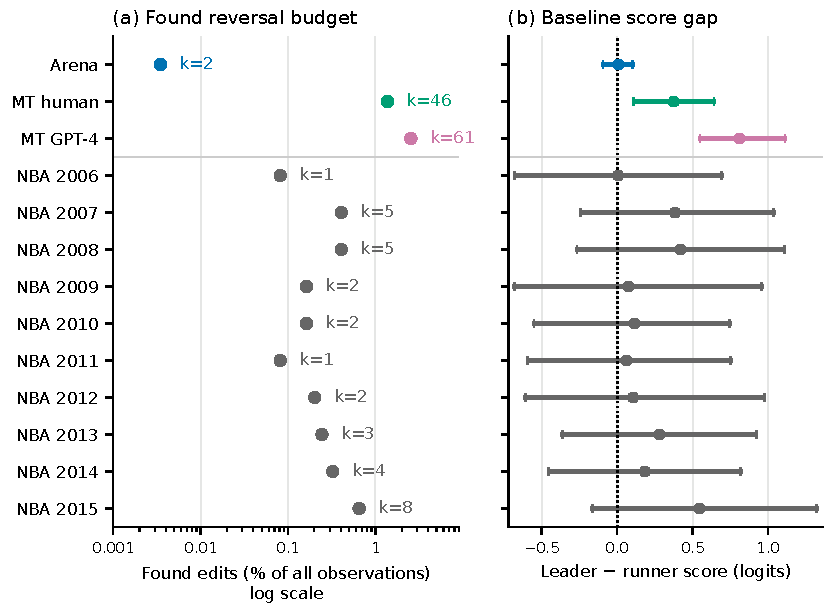
\includegraphics[width=\textwidth]{figures/primary_stability.pdf}
\caption{\FigPrimaryCaption}
\label{fig:primary}
\end{figure}

Figure~\ref{fig:primary} places the successful budgets alongside unedited leading-pair uncertainty.
The leading contrasts reverse after 2 Arena edits ($0.00348\%$), 46 human MT-Bench edits ($1.371\%$), and 61 GPT-4 MT-Bench edits ($2.542\%$). NBA found counts, in chronological order, are $1,5,5,2,2,1,2,3,4,8$, or $0.0813$--$0.6504\%$ of the corresponding season. Every count has a saved row-level witness and an exact-refit verification. These results demonstrate the existence of small successful changes; they do not estimate globally minimum budgets.

The uncertainty context changes their interpretation. Arena's original logit gap is $0.00813$, with a 95\% bootstrap percentile interval $[-0.09410,0.10430]$; its original leader loses first place in $45.4\%$ of unedited bootstrap fits. Every NBA leading-pair interval also spans zero. The human and GPT-4 MT-Bench intervals are $[0.10956,0.64196]$ and $[0.54993,1.11269]$, respectively. Thus the smallest found budgets accompany baseline leading contrasts that are already unresolved under the chosen resampling scheme. This is an observed association across these rankings, not a causal explanation or coverage guarantee.

\subsection{Targeting, random noise, and whole-rank change}

\begin{figure}[t]
\centering
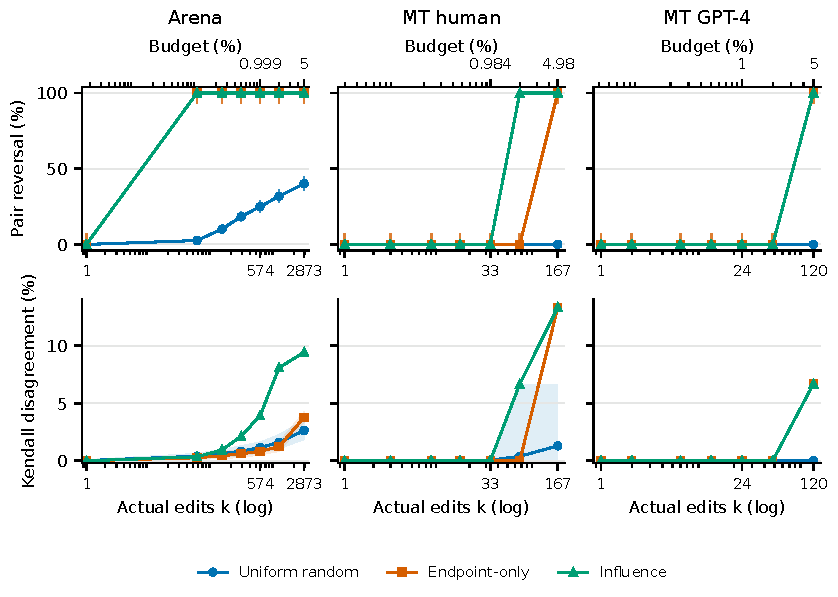
\includegraphics[width=\textwidth]{figures/strategy_curves.pdf}
\caption{\FigStrategyCaption}
\label{fig:strategy}
\end{figure}

Figure~\ref{fig:strategy} shows the measured budget curves; the full NBA panel is in Appendix~\ref{app:displays}.
At budgets near $1\%$ of all rows, both targeted strategies reverse Arena and all ten NBA original leading pairs. Random reversals do so in $25.0\%$ of Arena runs (Monte Carlo 95\% interval $21.3$--$29.0\%$) and $0$--$38.2\%$ of NBA runs. Neither MT-Bench leading pair reverses under any tested strategy at this budget. Zero of 500 random runs has an exact binomial upper endpoint of $0.735\%$; this concerns Monte Carlo frequency, not immunity to other edits.

First place and global order need different reporting. At the same Arena budget, influence targeting gives $D=0.0392$, endpoint targeting gives mean $D=0.00816$, and uniform random reversal gives mean $D=0.0114$. A targeted strategy can therefore reverse first place while changing fewer other orderings than random noise. In NBA 2006, random leading-pair reversal occurs in $38.2\%$ of runs while any winner change occurs in $38.6\%$; even these closely related endpoints are not identical. Budget fractions are rounded down to integer edits, so ``near $1\%$'' is nine games in the 990-game season, versus 12 in most other seasons.

\subsection{A shared-schedule human/model contrast}

\begin{figure}[t]
\centering
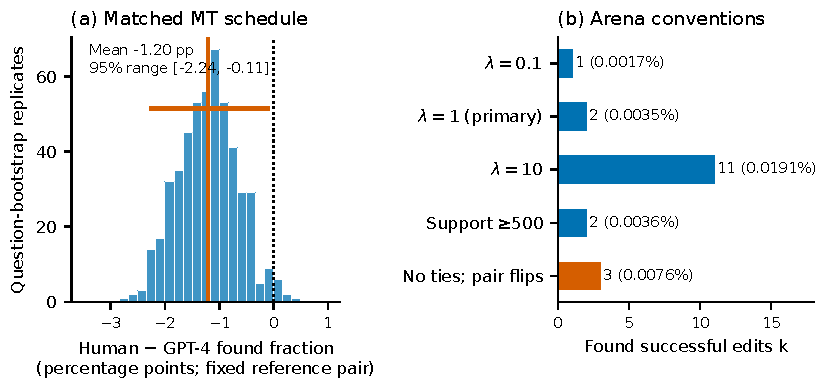
\includegraphics[width=\textwidth]{figures/controls.pdf}
\caption{\FigControlsCaption}
\label{fig:controls}
\end{figure}

Figure~\ref{fig:controls} displays the fixed-reference matched contrast and Arena convention checks.
On the fixed 1,814-cell support, every one of 100 human-label selections yields a smaller found top-two reversal fraction than GPT-4. Their mean difference is $-1.152$ percentage points. This variation conditions on the observed questions and concerns which human annotation is selected.

The joint question bootstrap gives a mean difference of $-1.243$ percentage points for the reselected-top-two statistic, with a percentile range $[-2.278,-0.110]$ points. However, GPT-3.5 replaces Claude-v1 as human runner-up in 106 of 500 replicates while GPT-4 remains leader; the human leader also changes in six. The post-hoc fixed GPT-4--Claude-v1 contrast avoids comparing a changing pair: its mean human-minus-GPT-4 found fraction is $-1.205$ percentage points, with range $[-2.244,-0.110]$. Humans have lower fractions in $98.2\%$ of replicates; five human replicates already reverse the reference pair and receive cost zero. All searches complete without censoring.

This shared-support result removes unequal row replication and observed schedule as explanations of this particular contrast. It still combines differences in labels, ties, fitted gaps and annotation dependence. Its percentile range describes a heuristic found-budget statistic; it is neither an interval for the optimal budget nor a general causal effect of human versus model judging.

\subsection{Modeling choices and sensitivity beyond first place}
Arena's found budget changes from one to two to eleven edits as $\lambda$ changes from 0.1 to 1 to 10. Restricting original incident support to at least 500 gives two edits. Removing ties changes the initial Arena leader and gives a three-edit reversal for the newly selected pair. These controls qualify any headline count: they change the specified estimator or population, and decisive-only fitting changes the target itself.

MT-Bench found counts remain unchanged across the tested ridge values. Expert-only humans yield 41 of 2,668 edits; excluding inconsistent GPT-4 ties yields 47 of 2,020. These are separate subsets, not repeated estimates of one unchanged quantity. The NBA home-advantage control retains every original leading pair and every found count, with all adjusted bootstrap intervals still spanning zero. Home adjustment addresses one omission; it does not remove temporal changes in strength.

The phenomenon also extends to other adjacent ranks. Exact refits demonstrate a one-edit reversal for 22 of Arena's 63 adjacent original pairs and 15--22 of 29 per NBA season. No MT-Bench adjacent pair has a single-edit reversal in the heuristic search. The positive counts establish existence; the negative search result does not certify absence.

\section{Discussion and limitations}
\label{sec:discussion}
A useful audit should accompany a successful-edit count with its starting margin and sampling uncertainty. When an unedited pair is poorly resolved, a tiny witness can reveal the fragility of its displayed order without showing that the underlying evaluation is invalid. When a contrast is better separated, the same fitted model may require substantially more edits. Our results support this joint reporting practice on the studied snapshots, while leaving general prediction of sensitivity open.

Comparing equal fractions alone is insufficient. One flipped game represents a larger share of a small season than one Arena battle, and a tied outcome enters the denominator without being editable. Participant count, comparison topology, ridge strength relative to sample size, and fitted gaps all matter. The matched MT-Bench analysis makes one comparison more controlled, but does not identify a design-level causal effect. Nor does our selected-pair heuristic establish worst-case stability of an entire ranking. Exhaustive optimization or certified lower bounds would answer a stronger question and are not supplied.

Our intervention assumes the ability to revise existing decisive labels with full data access. Real attackers may submit new votes under authentication, sampling and rate constraints; accidental errors may follow correlated mechanisms rather than uniform flips. We evaluate neither setting directly. We also preserve all ties, use a static fractional-tie Bradley--Terry model, and study a limited collection of historical snapshots. Bootstrap clusters approximate available dependence and cannot recover missing users, fully crossed annotators, or evolving team strength. Selection of the original top pair and the post-hoc fixed-reference control limit interval interpretation.

These diagnostics can improve evaluation transparency, while the same targeting ideas could guide selective corruption where historical outcomes are editable. We release code and aggregate evidence for public snapshots, without implementing platform submissions or redistributing raw conversations and full source datasets. Minimal processed outcome rows support witness verification. The practical implication is to expose uncertainty and specification dependence alongside a rank, and to retain reproducible witnesses for concrete sensitivity claims. Sensitive witnesses should be understood as diagnostics under a declared intervention. They do not by themselves establish compromised votes, an exploitable platform, or that a different judging design would fix the observed sensitivity.

\section{Conclusion}
Across public preference and sports data, successful label reversals range from a few outcomes to several percent, and the smallest found budgets coincide with unresolved bootstrap leading contrasts. Shared-schedule MT-Bench results retain a descriptive difference between human and GPT-4 labels, while robustness controls show that a single sensitivity number depends on modeling choices. Explicit endpoints, exact refits, saved witnesses, and separate accounts of perturbation and sampling uncertainty make these conclusions checkable without treating heuristic searches as certificates.
